% Source page: original p. 335 (PDF p. 31)
% Figure number: Figure 14
% Uncertainty notes: VERIFY: the contour waviness and the exact right-end drop are slightly blurred in the scan; this redraw matches the visible geometry but may merit a final side-by-side recheck.
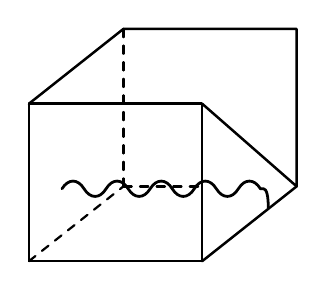
\begin{tikzpicture}[x=1cm,y=1cm,line cap=round,line join=round]
  % Front face
  \coordinate (A) at (0.00,0.00);
  \coordinate (B) at (2.20,0.00);
  \coordinate (C) at (2.20,2.00);
  \coordinate (D) at (0.00,2.00);
  \coordinate (E) at (1.20,0.95);
  \coordinate (I) at (2.20,0.95);
  \coordinate (F) at (3.40,0.95);
  \coordinate (G) at (3.40,2.95);
  \coordinate (H) at (1.20,2.95);

  % Visible outer cube
  \draw[line width=0.9pt] (A) -- (B) -- (C) -- (D) -- cycle;
  \draw[line width=0.9pt] (D) -- (H) -- (G) -- (F) -- (C);
  \draw[line width=0.9pt] (B) -- (F);

  % Hidden edges
  \draw[dashed,line width=0.8pt] (H) -- (E);
  \draw[dashed,line width=0.8pt] (E) -- (I);
  \draw[dashed,line width=0.8pt] (A) -- (E);

  % Wavy contour through the box
  \draw[line width=1.0pt]
    (0.42,0.92)
    .. controls (0.50,1.05) and (0.62,1.05) .. (0.70,0.92)
    .. controls (0.78,0.79) and (0.90,0.79) .. (0.98,0.92)
    .. controls (1.06,1.05) and (1.18,1.05) .. (1.26,0.92)
    .. controls (1.34,0.79) and (1.46,0.79) .. (1.54,0.92)
    .. controls (1.62,1.05) and (1.74,1.05) .. (1.82,0.92)
    .. controls (1.90,0.79) and (2.02,0.79) .. (2.10,0.92)
    .. controls (2.18,1.05) and (2.30,1.05) .. (2.38,0.92)
    .. controls (2.46,0.79) and (2.58,0.79) .. (2.66,0.92)
    .. controls (2.74,1.05) and (2.86,1.05) .. (2.94,0.92)
    -- (2.98,0.92)
    .. controls (3.02,0.92) and (3.04,0.82) .. (3.04,0.68);
\end{tikzpicture}
